%\documentclass{article} % For LaTeX2e

\documentclass[letterpaper, 10 pt, conference]{ieeeconf}  % Comment this line out if you need a4paper
%\documentclass[a4paper, 10pt, conference]{ieeeconf}      % Use this line for a4 paper
\IEEEoverridecommandlockouts                              % This command is only needed if you want to use the \thanks command
\overrideIEEEmargins

%\usepackage{nips13submit_e,times}
\usepackage{hyperref}
\usepackage{url}
\usepackage{graphicx}
\usepackage{amsmath}
\usepackage{wrapfig}
\usepackage[font=scriptsize]{caption}
\usepackage{color}
%\documentstyle[nips13submit_09,times,art10]{article} % For LaTeX 2.09


\title{\LARGE \bf Robust Graph SLAM in Dynamic Environments with Moving Landmarks}


\author{Lingzhu Xiang$^{1}$ \and Zhile Ren$^{1}$ \and Mengrui Ni$^{1}$ \and Odest Chadwicke Jenkins$^{1}$
\thanks{$^{1}$Lingzhu Xiang, Zhile Ren, Mengrui Ni, and Odest Chadwicke Jenkins are with the Department of Computer Science, Brown University, Providence, RI 02912 {\tt\small [xlz$|$ren$|$mni$|$cjenkins]@cs.brown.edu} 
}
}

% The \author macro works with any number of authors. There are two commands
% used to separate the names and addresses of multiple authors: \And and \AND.
%
% Using \And between authors leaves it to \LaTeX{} to determine where to break
% the lines. Using \AND forces a linebreak at that point. So, if \LaTeX{}
% puts 3 of 4 authors names on the first line, and the last on the second
% line, try using \AND instead of \And before the third author name.

\newcommand{\fix}{\marginpar{FIX}}
\newcommand{\new}{\marginpar{NEW}}

\newcommand{\cj}[1]{{\color{red} \bf CJ: #1} }
%\long\def\chad#1{\colorbox{yellow}{\bf \small *CJ: #1*}}

%\nipsfinalcopy % Uncomment for camera-ready version

\begin{document}


\maketitle
\thispagestyle{empty}
\pagestyle{empty}


%A clear description of the problem or application you intend to address. Why is it worth studying?
%A discussion of related work, including references to at least three relevant research articles or technical reports. Which aspects of your project are novel?
%A figure illustrating a preliminary experiment with some data related to your project. This could be some sort of visualization of the raw data, or the results of running a simple (supervised or unsupervised) machine learning method.
%A description of the learning and/or inference challenges that you need to solve to apply a graphical model to your data. It is fine if you do not yet know what algorithms are appropriate, but discuss the challenges that need to be solved.
%An experimental evaluation protocol. How will you know that you've succeeded?
%A concrete timeline for accomplishing your project by the end of the course. What are the biggest challenges?

\begin{abstract}
Recent developments in human-robot interaction bring about higher requirements
for robot navigation. Existing Simultaneous Localization and Mapping (SLAM)
algorithms have become unsuited for navigation in complex dynamic
environments due to presumptions of static environments or exceeding
computational limitations. In this paper we propose a new graph SLAM framework
exploring incremental EM algorithms to maintain a reference frame while
establishing the estimations of robot trajectory and the map in real-time. We
plan to evaluate the performance of existing robust SLAM algorithms as baselines,
and validate the improvement of our new framework against datasets of dynamic
environments with moving objects.
\end{abstract}

\section{Introduction}
Simultaneous localization and mapping (SLAM) is a central problem for
autonomous robot navigation. \cj{*run on sentence, split* Graph SLAM formulate it as an inference problem
on a factor graph, where landmark locations and robot poses are the hidden
variables nodes to be mapped and localized, and spatial measurements are the
observed factor nodes as constraints between variable nodes.} The goal of
the inference problem is to obtain the maximum likelihood estimate of the
joint probability of the graph, which becomes the geometrically consistent
estimate of the robot's trajectory and the map. This maximum likelihood estimate on factor graphs can be solved by belief propagation \cj{perhaps cite Weiss et al.}, or more recently, by numerical methods after converting into a nonlinear squares optimization \cj{cite iSAM?}.  

Problems arise in SLAM loop closures when factors incorrectly link unrelated variable nodes.  Such false positives effectively create wormholes between spatially distant locations and, thus, distort the map geometry. In pose graphs, loop closures specify spatial localities between arbitrary poses, but often wrongly connect randomly poses because of bad decisions from the front-end.  In landmark-based graphs, the data association process can also easily obtain wrong visual feature correspondences, connecting landmarks to the wrong poses. This necessitates robust SLAM.

Another issue beyond robust SLAM is dynamic elements in the environment.
Typical SLAM techniques in the literature are designed for unmanned navigation
in uninhabited areas, thus mostly assume static environments with stationary
landmarks or loop closures. However, recent human-robot interaction research
has seen more applications of navigation in populated, crowded, or social
environments where people and furniture moving around is the major
characteristics. If the landmarks are moving, the current localization is either
kidnapped by the movement, or resulting in distorted maps.

In this paper we devise new graph representations and algorithms to
address the issue of front-end outliers and the issue of environmental
dynamic elements within the factor graph framework. We evaluate existing
approaches of robust SLAM and conduct experiments on real world datasets to
validate the performance of our approach.

\section{Related Work}

Graph SLAM has multiple highly efficient optimization solutions.
iSAM \cite{isam} converts the graph SLAM maximum likelihood estimate into a
non-linear least squares optimization problem.  The factor graph is incrementally solved by numerical methods, obtaining real-time performance and Bayesian smoothing accuracy. These optimization techniques show the effectiveness of the factor graph formulation of the SLAM problem, and we base our formulation on similar formulations.

\cj{let's also look at Wolf and Sukhatme, http://robotics.usc.edu/publications/media/uploads/pubs/392.pdf}

A known solution to moving objects in the environment is combining SLAM with
object detection and tracking. \cite{wang2003online} proposes a Bayesian
framework to solve the SLAM together with object motion modeling by
sophisticated object detection and tracking and data association algorithms.
This approach is suitable for dense data such as laser point-clouds, but less
so for sparse data such as landmarks or features keypoints generated by visual
sensors which is usually less than sufficient to achieve the same level of
accuracy.  Moreover, object detection and tracking is used as a preprocessing
front-end to filter out moving objects. If the goal is just to estimate the
robot trajectory and the still part of the map for future localization, the
work of maintaining motion models of individual moving objects will not be
essential to the SLAM problem. 

Robust SLAM techniques have been proposed to solve front-end outlier problems
without relying on pre-filtering. Some use robust objective functions or robust
representation of observations. Dynamic Covariance Scaling\cite{DCS} adds a
robust kernel factor to regularize the Mahalanobis errors in the Gaussian
distributions of landmark observations.  Max-Mixture\cite{mm} enhances factor
representation with a mixture of Gaussians instead of a single spatial Gaussian
distribution. This kind of approaches still assume sources of errors being
mostly perceptual aliasing in wrong loop closures, without regard to
environmental movement.  Given dynamic environments they will have difficulty
in detecting and handling the movement of landmarks.

The other approach to handling front-end outlier and dynamic elements is
incorporating the problem of identifying mobility as part of the back-end graph
optimization framework.  \cite{haehnel03iros} and \cite{rogers2010slam} extend
the graphical model with a latent indicator variable for each landmark to
indicate whether it is mobile and use EM algorithms to iteratively infer those
additional latent variables in the graphical model and estimate the optimal
solution in SLAM augmented with the indicators. The switchable
constraints \cite{Switchable12} approach allows the optimizer to naturally
change the topological structure of the problem during the optimization itself
using switch variables as a multiplicative scaling factor on the information
matrix associated with that constraint. However, these EM based algorithms lack
the robustness provided by previous techniques.  And observation based
indicators will not be able to characterize the mobility of each landmark which
associates with multiple observations.

\section{Graphical Model Formulation}
The graphical model formulation of our approach is shown in figure \ref{fig:model}. 
\begin{figure}[h]
\begin{center}
%\framebox[4.0in]{$\;$}
%\fbox{\rule[-.5cm]{0cm}{4cm} \rule[-.5cm]{4cm}{0cm}}
 \includegraphics[width=0.5\linewidth]{fig/model} 
\end{center}
\caption{Graphical Model Formulation}
\label{fig:model}
\end{figure}

\section{ALGORITHMS}
Following the notation in section \ref{sec:model}, we introduce the Expectation Maximization (EM) algorithms for estimating $w$ with robustified objective function to learn the mobility of landmarks and estimate the robot trajectory and the map.

\subsection{Estimation of Latent Parameters}
\label{sec:traditionalEM}

As described in \cite{rogers2010slam}, in Equation \ref{eq:sensor}, the hidden variables $w_k$ must be estimated from multiple observations of each landmark. In the \textbf{M step}, we select the optimal $w$ which maximizes the joint likelihood. However there is a trivial solution to the likelihood maximization which sets $w_k = 0$ for all $k$, we penalize the log-likelihood objective in Equation \ref{eq:lagrangeMultiplier} with Lagrange multiplier which act as priors of the latent landmark mobility variables:
\begin{multline}
%\begin{aligned}
\mathrm{Obj}(Z, X, L, W) = \\ \sum_k \left[ -w_{j_k}(\tilde{\mu}^T_k\Sigma_k^{-1}\tilde{\mu}_k) \right] - \frac{1}{2}\lambda(1 - w)^T(1 - w)
%\end{aligned}
\label{eq:lagrangeMultiplier}
\end{multline}
where $\tilde{\mu}_k = v_k (h_k(x_{i_k}, l_{j_k}) - z_k)$ is the robustified prediction error of observation $k$ obtained from the E step, and $w_{j_k}$ is the weight to estimate for landmark $l = j_k$ associated with the $k$-th observation. We equate the derivative of the objective function with respect to $w_l$ to zero, and maximize the log likelihood, then for each $w_l$ we get
\begin{equation}
\begin{aligned}
w_l = 1 - \frac{1}{\lambda} \sum_{k \in K_l}\tilde{\mu}^T_k\Sigma_k^{-1}\tilde{\mu}_k
\end{aligned}
\label{eq:wk}
\end{equation}
where $K_l$ is the set of measurements of landmark $l$, and $\lambda$ is an assigned constant parameter to trade off the penalty. Larger $\lambda$ will penalize more against the number of landmarks being mobile $w_k = 0$ for any $k$.

\subsection{Graph SLAM Optimization}

In the \textbf{E step}, we use the estimated latent parameters to obtain minimum variance results with graph optimization methods. We employ the standard approach of graph optimization as in \cite{g2o}, with our augmentation to the objective by introducing landmark mobility indicators $w_{j_k}$ and observation robust kernel $v_k$. Specifically, we want to compute the maximum likelihood estimate of the robust objective
\begin{equation}
\begin{aligned}
X^*, L^* = \operatorname*{arg\,max}_{X, L} & \{ -\log p(X, L, U, Z, W) \}\\
=\operatorname*{arg\,max}_{X, L} & \{ \sum_{i=1}^M||f_i(x_{i-1}, u_i) - x_i)||^2_{\Gamma_i} \\
&+ \sum_{k=1}^K w_{j_k}|| v_k (h_k(x_{i_k}, l_{j_k}) - z_k)||^2_{\Sigma_k} \\ 
&+ \sum_{k=1}^K ||1 - v_k||^2_{\Xi_k} \}
\end{aligned}
\label{eq:MAP}
\end{equation}
where the $||.||_\Sigma$ term denotes the Mahalanobis distance with covariance $\Sigma$. The penalty term $|| 1 - v_k||^2_{\Xi_k}$ here is the switching prior introduced in \cite{Switchable12}. Note that in this step, $w$ is fixed and the penalty term with respect to $w_k$ in the objective for estimating $w$ becomes a constant, thus it does not appear in the objective function.

Here we apply the Dynamic Covariance Scaling\cite{DCS} kernel $v_k$ to each individual observation $k$. The factor $v_k$ for observation $k$ is given as:

\begin{equation}
\begin{aligned}
v_k = \min \left\{ 1, \frac{2\Phi}{\Phi + w_{j_k}\mu_k^T \Sigma_k^{-1} \mu_k}\right\}
\end{aligned}
\label{eq:DCS}
\end{equation}

where $\mu_k = h_k(x_{i_k}, l_{j_k}) - z_k$ is the original prediction error of observation $k$. The DCS kernel is shown to result in an upper bound specified by $\Phi$ for the second part of the objective function. By specifying the upper bound $\Phi$ for all robust edges, $v$ dynamically scales the information matrices of all edges each iteration within the graph optimization process, and replaces the covariances of outliers with large ones making it near uniform. $\Phi$ is chosen as 1 in our implementation as suggested by its author. 

With some derivation %\footnote{See Appendix section \ref{appendix:leastsquare} for detail.}
(Appendix section), the optimization problem can be formed as a standard least-squares problem:
%resolved\cj{why the subscript covariance $_2$? xlz: removed $_2$, this is just plain L2-norm}

\begin{equation}
\delta^* = \operatorname*{arg\,max}_\delta||A\delta - b||^2
\label{eq:optimization}
\end{equation}


The algorithm, while reliable as shown in experiments in \cite{haehnel03iros}, is possible to have variants modified for real-time updates. In our current implementation we perform batch optimization. We need to rerun the EM algorithm if new measurements are observed. Incremental implementation of the framework is subject for future work.

\subsection{Incremental Optimization}
We introduce the theoretical basis for an incremental implementation of the EM algorithm for the problem. As suggested in \cite{neal1998EM}, if the joint probability is fully factorized with regards to the examples, as is in our case, we can use the following algorithm for update in the E and M step while preserving the correctness:

\paragraph{E step} 
In equation \ref{eq:MAP}, if we have one new observation $z_{K+1}$ at time $K+1$, then

\begin{equation}
\begin{aligned}
x_{i_{K+1}}^*, l_{j_{K+1}}^*  
&= \operatorname*{arg\,max}_{ x_{i_{K+1}}, l_{j_{K+1}}} \{ 
\sum_{i}||f_i(x_{i-1}, u_i) - x_i)||^2_{\Gamma_i} \\
&\hspace{0.5cm}+ \sum_{k=1}^{K+1} w_{j_k}||v_k(h_k(x_{i_k}, l_{j_k}) - z_k)||^2_{\Sigma_k} \\ 
&\hspace{0.5cm}+ \sum_{k=1}^{K+1}||1-v_k||^2_{\Xi_k} \}
%&= \operatorname*{arg\,max}_{ x_{i_{K+1}}, l_{j_{K+1}}} \{ 
%\sum_{i}||f_i(x_{i-1}, u_i) - x_i)||^2_{\Gamma_i} \\
%&+ \sum_{k=1}^{K+1} w_{j_k}||v_k(h_k(x_{i_k}, l_{j_k}) - z_k)||^2_{\Sigma_k} \\
%&+ \sum_{k=1}^{K+1}||1-v_k||^2_{\Xi_k} \}
\end{aligned}
\label{eq:facMAP}
\end{equation}

and equation \ref{eq:facMAP} can also be written in the form of \ref{eq:optimization}, but with less parameters. So, the incremental E step becomes
\begin{itemize}
\item Choose one observation term $k$ to be updated, such as $k = K+1$
\item Set $x_{i_p}^{(t)} = x_{i_p}^{(t-1)}, l_{j_p}^{(t)} = l_{j_p}^{(t-1)}$ for $p \neq k$
\item Set $x_{i_k}, l_{j_k}$ according to equation \ref{eq:MAP} in equation \ref{eq:optimization}'s form.
\end{itemize}
\paragraph{M step} The same step as introduced in section \ref{sec:traditionalEM}, using the derivation in equation \ref{eq:wk}.

With this incremental EM algorithm, the E step can be much faster since the optimization problem has less parameters. Also, after several iterations, we may use the model to update the parameters by adding more observations, without the need to run the EM algorithm on all the observations again.

\section{Preliminary Results}

In this section, we evaluate the performance of the state-of-the-art robust
SLAM method, the Max-Mixture algorithm, given dynamic landmark measurements.
Max-Mixture is a robust extension to classical graph SLAM using Gaussian
mixture in factor representation, that is, $ x_i = \sum_c \phi_c
\mathcal{N}(\mu_c, \Sigma_c)$ for component $c$ and weight $\phi_c$, with
obvervations being components, also similarly for $z_i$. Max-Mixture uses a max
function to approximate and efficiently evaluate the sum of Gaussians. It is
well-known for its capability of handling a large amount of incorrect loop
closures, but it is untested against moving landmarks, and this experiment can
be representative to other approaches in the robust SLAM literature. 

We apply different perturbations to a single landmark (landmark 249) in the
Victoria Park dataset, and compare the different effects of the perturbations
on the optimal estimate of the trajectory and the map of all landmarks obtained
by Max-Mixture graph SLAM. The Victoria Park dataset contains 2-D odometry and
landmark observations. As shown in figure \ref{fig:baseline} the left plot is
the control group without perturbation, and is accurate to the ground truth. A
single southward bias is applied to all observations of the
landmark in the middle plot, simulating sensory outliers. A temporally
increasing bias is applied to all observations of the landmark in the right
plot, simulating a southward moving landmark.

\begin{figure}[h]
\makebox[\textwidth][c]{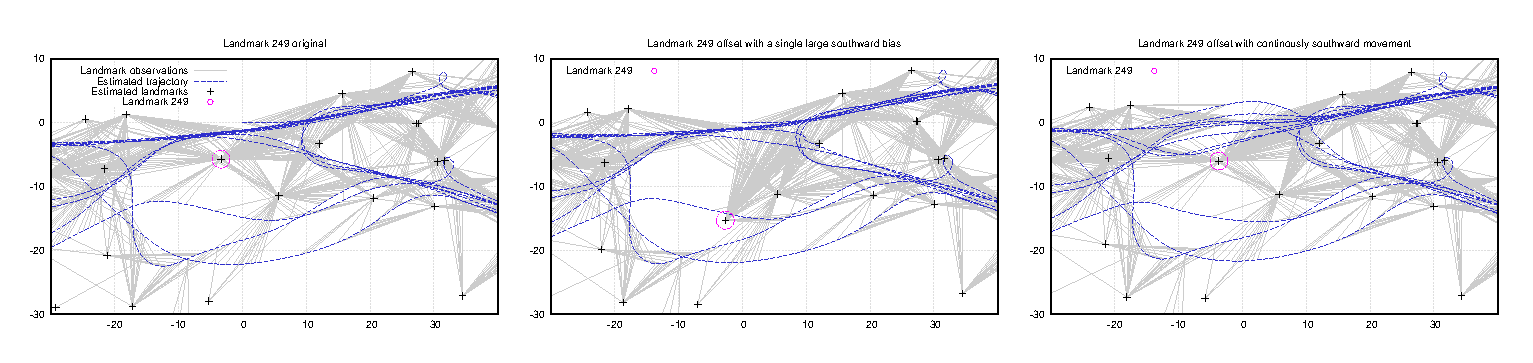
\includegraphics[width=\textwidth]{fig/baseline-mm}}
\caption{The optimal estimates of the trajectory and landmark positions
obtained by Max-Mixture graph SLAM.  Left: low convergence uncertainty. Middle:
high convergence uncertainty because of rejection of outlier observations
of landmark 249.  Right: low convergence uncertainty, no outlier
detected by Max-Mixture.}
\label{fig:baseline}
\end{figure}

As the middle plot shows, Max-Mixture is still capable of handling noise of
large bias or spurious loop closures introduced by simluated sensory fault. It
correctly rejects outlier landmark observations and recovers the position of
the perturbed landmark. However, it completely fails to reject any unlikely
landmark observations and largely distorts the resulting trajectory when given
moving landmark measurements. An explanation for this is that each clique of
landmarks with coherent motion forms a plausible reference frame for related
observations. Inference based on each independent reference frame will reach
plausible estimate of robot trjectory and the map, however robust SLAM methods
which assume stationary landmarks will average over a sum of different
reference frames and lead to wrong conclusions.


\section{DISCUSSION AND FUTURE WORK}

We have shown the basic efficacy of our approach, but the evaluation is far from being comprehensive. The performance under different percentage of randomly generated outliers, and different sources and types of datasets including 3-D datasets are needed for a complete understanding of the performance in our approach. Due to the different nature of source of errors of moving landmarks than spurious loop closure, the effect of different numbers of observations associated with landmarks also needs to be taken into account for systematic evaluation.

We have examined the theoretical basis for the incremental variant of the EM algorithms. Considering the fast convergence of our batch EM algorithm it might be possible to integrate the incremental algorithm into the graph optimization process without loss of the correctness of the EM algorithms, and making our approach suitable for real-time update.

In our formulation, there are pre-defined parameters $\lambda$ for penalizing against removing too many landmarks, which is essentially a decision boundary, and $\Phi$ for the robust kernel. The appropriate method to choose the parameters and their sensitivity to environmental factors and dataset characteristics need to be examined. There are multiple robust SLAM methods proposing different penalty terms which derive into these parameters. A comparison of the alternative choices of penalty terms is also necessary.

\section{CONCLUSION}

This paper proposed a new method to characterize and identify the mobility of potentially moving landmarks by using the EM algorithms with robust kernel. The feasibility of the proposed approach was shown and evaluated on synthesized datasets from a standard dataset. We compared with existing state-of-the-art methods and showed that observation based robust methods are unable to handle moving landmarks while EM alone without robust kernel does not deal with small continuous movement robustly. We also propose an incremental variant of our approach which will be suitable for real-time incremental update in future implementation.

%\subsection*{Author Contributions Statement}
%Xiang, Ni, and Ren developed the concept of the model. Xiang and Ni surveyed the literature. Ren provided mathematical derivation and the figure. Xiang implemented the algorithm and data processing utility. Xiang and Ni designed and performed experiments. Xiang provided the experiment visualization. Xiang drafted and finalized the majority of the manuscript; Ren drafted the derivation; Ni drafted a subsection in Related Work and a subsection in Experimentation.

%\newpage
\appendix
\subsection{SLAM as a Least Squares Problem}
\label{appendix:leastsquare}
For completeness of the paper, we review how to form the SLAM optimization problem as a least squares problem, following the derivation in \cite{isam}. Recall that in equation \ref{eq:MAP}, we need to solve a quadratic program, however we may approximate the terms with first order polynomials. For the process term,
\begin{equation}
\begin{aligned}
f_i(x_{i-1}, u_i) - x_i\\
\approx & {f_i(x_{i-1}^0, u_i)} + F_i^{i-1}\delta x_{i-1} - (x_i^0 + \delta x_i)\\
=& F_i^{i-1}\delta x_{i-1} + G_i^i\delta x_i - a_i \\
\end{aligned}
\label{eq:linearProcessTerm}
\end{equation}
where $I$ is the identity and %resolved\cj{does $I$ refer to the matrix identity? define xlz: yes}
\begin{equation*}
\begin{aligned}
F_i^{i-1} &= \frac{\partial f_i(x_{i-1}, u_i)}{\partial x_{i-1}}|_{x_{i-1}^0}, \label{F} \\%\quad
 G_i^i &= -I, \text{(Identity matrix)}\\% \quad 
a_i &= x_i^0 - f_i(x_{i-1}^0, u_i).
\end{aligned}
\end{equation*}
For the measurement term:
\begin{equation}
\begin{aligned}
h_k(x_{i_k}, l_{j_k}) - z_k\\
\approx & {h_k(x_{i_k}^0, l_{j_k}^0) + H_k^{i_k}\delta x_{i_k} + J_k^{j_k}\delta l_{j_k}} - z_k\\
= & {H_k^{i_k}\delta x_{i_k} + J_k^{j_k}\delta l_{j_k}} - c_k\\
\end{aligned}
\label{eq:linearMeasurementTerm}
\end{equation}
where, %resolved\cj{What is the difference between $H_k^{i_k}$ and $J_k^{j_k}$? Should $J_k^{j_k}$ be with respect to $x_{j_k}$? xlz: fixed, the denominator of $J$ should be $l_{j_k}$}
\begin{equation*}
\begin{aligned}
H_k^{i_k} &= \frac{\partial h_k(x_{i_k}, l_{j_k})}{\partial x_{i_k}}|_{(x_{i_k}^0, l_{j_k}^0)}, \\ 
J_k^{j_k} &= \frac{\partial h_k(x_{i_k}, l_{j_k})}{\partial l_{j_k}}|_{(x_{i_k}^0, l_{j_k}^0)} , \\
 c_k &= z_k - h_k(x_{i_k}^0, l_{j_k}^0)
\end{aligned}
%\label{eq:linearMeasurementTerm}
\end{equation*}
%In our case, 
%\begin{equation}
%\begin{aligned}
%h(x_i, l_j) = 
%\begin{pmatrix}
%\sqrt{(x_i^x - l_j^x)^2 + (x_i^y - l_j^y)^2}\\
%\tan^{-1}(\frac{l_j^y - x_j^y}{l_j^x - x_i^x}) - \theta_i
%\end{pmatrix}\\
%\end{aligned}
%\label{eq:measurementTermDerivative}
%\end{equation}


Therefore, the optimization problem thus becomes
\begin{equation}
\begin{aligned}
\delta \theta^* = 
\operatorname*{arg\,min}&_{\delta \theta}\{\sum_{i=1}^M||F_i^{i-1}\delta x_{i-1} 
+ G_i^i\delta x_i - a_i||_{\Gamma_i}^2 \\ 
&\hspace{-0.5cm}+ \sum_{k=1}^Kw_{j_k}||v_k(H_k^{i_k}\delta x_{i_k} 
 + J_k^{j_k}\delta l_{j_k} - c_k)||_{\Sigma_k}^2\}
\end{aligned}
\end{equation}

To rewrite the Mahalanobis norm, notice that
\begin{equation}
||e||_{\Gamma}^2 = e^T\Gamma^{-1}e = ||\Gamma^{-T/2}e||^2
\end{equation}

Therefore, we can collect all the Jacobian matrices multiplied by either $\Gamma_i^{-T/2}$ or $v_k w_{j_k}^{1/2}\Sigma_k^{-T/2}$, specifically,

\begin{equation}
\begin{aligned}
\delta \theta^* =& \operatorname*{arg\,min}_{\delta \theta}\{&
\\ &\sum_{i=1}^M||\Gamma_i^{-T/2}F_i^{i-1}\delta x_{i-1} + \Gamma_i^{-T/2} G_i^i\delta x_i - \Gamma_i^{-T/2}a_i||^2  \\
&+\sum_{k=1}^K||v_k\sqrt{w_{j_k}}\Sigma_k^{-T/2} H_k^{i_k}\delta x_{i_k} 
\\ &\hspace{0.5cm}+ v_k\sqrt{w_{j_k}}\Sigma_k^{-T/2}J_k^{j_k}\delta l_{j_k} 
- v_k\sqrt{w_{j_k}}\Sigma_k^{-T/2}c_k||^2\}
\end{aligned}
\end{equation}

We concatenate the matrices $F, G, H, J$ in block form into a square matrix $A$, $\delta x, \delta l$ into $\delta \theta$, and $a$ and $c$ into the residual vector $b$ to then obtain the standard least squares problem:
\begin{equation}
\delta \theta^* = \operatorname*{arg\,min}_{\delta \theta}||A\delta \theta - b||^2
\end{equation}


%\section{ACKNOWLEDGEMENTS}

%\bibliographystyle{plain}
\bibliographystyle{IEEEtranS}
\bibliography{cs242_slam}{}
%\subsection{Figures}
%\begin{figure}[h]
%\begin{center}
%%\framebox[4.0in]{$\;$}
%\fbox{\rule[-.5cm]{0cm}{4cm} \rule[-.5cm]{4cm}{0cm}}
%\end{center}
%\caption{Sample figure caption.}
%\end{figure}


\end{document}
